\section{Quick Tutorial}

The best way to get started with JOD is to work through the
lab\index{labs} \emph{JOD (1) Introduction}.\footnote{
The number ``($n$)'' in JOD lab titles is a suggested order.}
JOD labs are listed in the \texttt{General} category: see 
Figure~\ref{eps:jodlabs} on page~\pageref{eps:jodlabs}.  This tutorial
uses lab material; work through the JOD labs after reading this section.

%Down in the hard-core cyber trenches, away from the glittering GUIs and sexy web interfaces, you will find command-lines.  
% This
%tutorial introduces a handful of JOD words.  To see the complete
%list of JOD words see section~\ref{ss:jodwords} on page~\pageref{ss:jodwords}.

\begin{figure}[htbp]
  \centering
  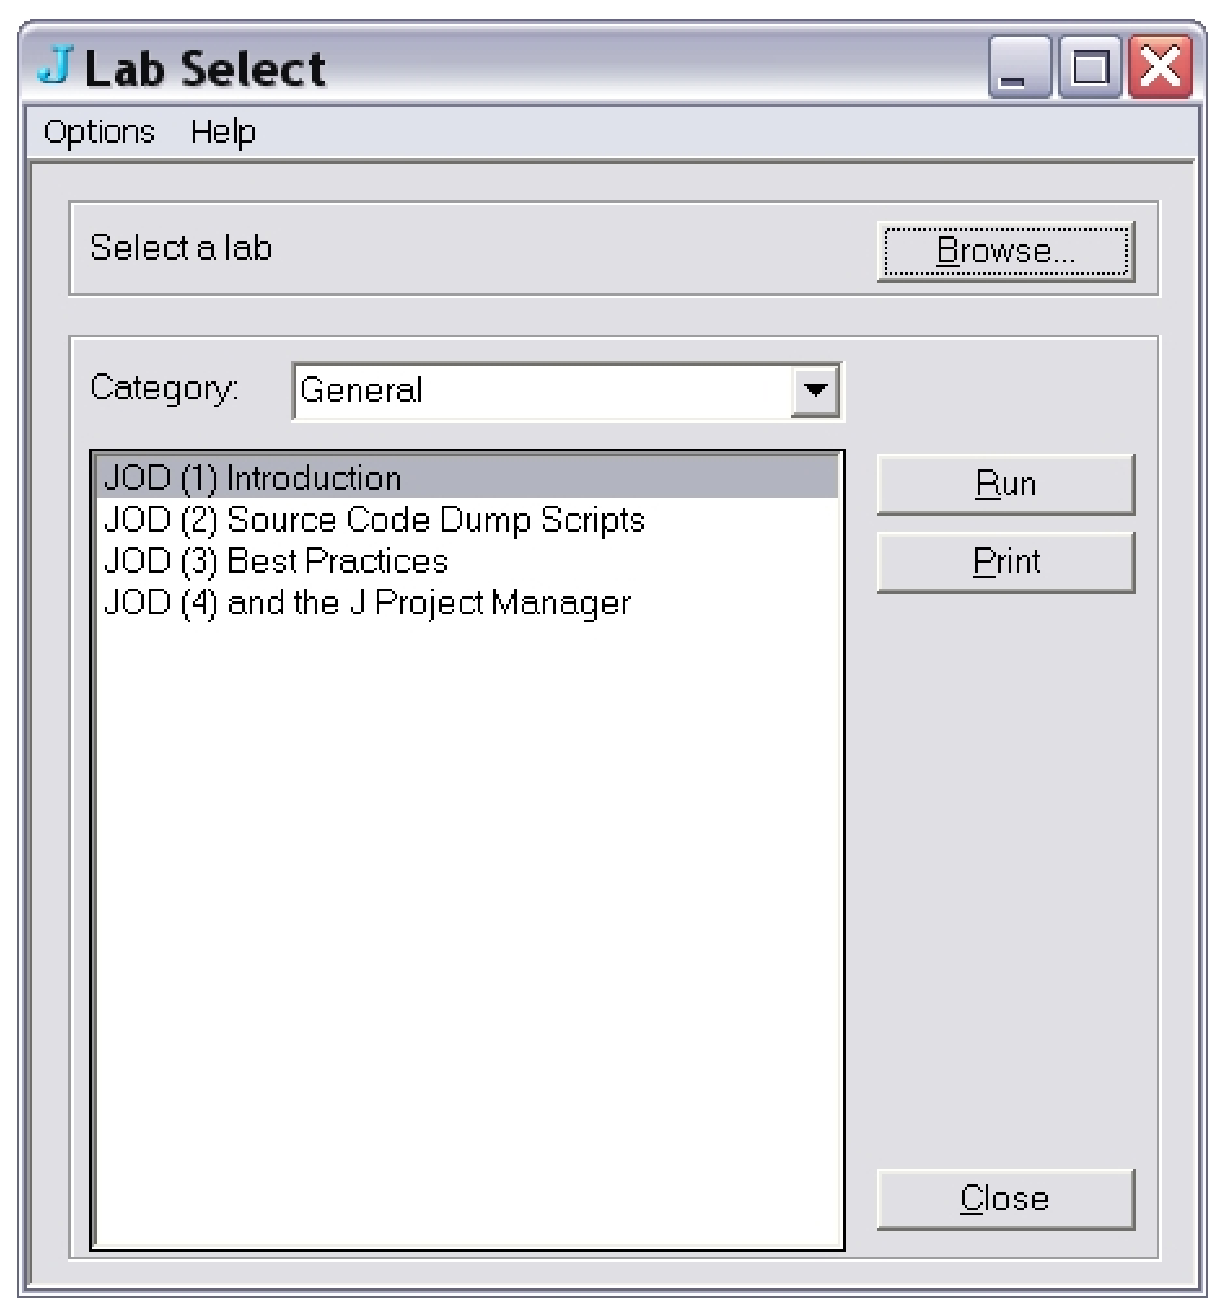
\includegraphics[width=0.60\textwidth]{jodlabs}
  \caption[JOD Labs]{JOD Labs are installed in the \texttt{General} category.}
   \label{eps:jodlabs}
\end{figure}

%JOD is primarily and old-fashioned command-line system. Command-line
%computing still reigns supreme in the \emph{productive} nether-worlds of software.
%J is  a magnificient example of a command-line system.  You can rule
%your computing universe with a few well considered lines of J: see Figure~\ref{eps:ziggy}
%on page~\pageref{eps:zippy}. JOD is
%designed to run in a J session and augment J.

\begin{description}
\item[Start JOD.]  After installation JOD can be started from a J session with:
\begin{lstlisting}[frame=single,framerule=0pt]
   require 'general/jod'   NB. start JOD 
\end{lstlisting}


\item[Create dictionaries.] To use JOD you must create some dictionaries
with \hyperlink{il:newd}{\texttt{newd}}: see page~\pageref{ss:newd}.
JOD words, with a few exceptions, return boxed list results.  The first
item is a return code where \texttt{1} indicates success and \texttt{0} means failure.
\begin{lstlisting}[frame=single,framerule=0pt]
   newd 'lab';'c:/jodtut/lab'   NB. create (lab)
+-+---------------------+---+--------------+
|1|dictionary created ->|lab|c:/jodtut/lab/|
+-+---------------------+---+--------------+

   newd 'labdev';'c:/jodtut/labdev'  NB. create (labdev)
+-+---------------------+------+-----------------+
|1|dictionary created ->|labdev|c:/jodtut/labdev/|
+-+---------------------+------+-----------------+
\end{lstlisting}

\item[Open dictionaries.] To use a dictionary it most be open. Open
dictionaries with \hyperlink{il:odd}{\texttt{od}}: see page~\pageref{ss:od}.
\begin{lstlisting}[frame=single,framerule=0pt] 
   od 'labdev'    NB. open read/write
+-+--------------+------+
|1|opened (rw) ->|labdev|
+-+--------------+------+
 
   2 od 'lab'     NB. open read/only
+-+--------------+---+
|1|opened (ro) ->|lab|
+-+--------------+---+
\end{lstlisting}

\item[Show open dictionaries.] Open dictionaries define a \emph{reference path}, see
appendix~\ref{ap:refpath} on page~\pageref{ap:refpath}. \hyperlink{il:did}{\texttt{did}}, see page~\pageref{ss:did}, displays information about open dictionaries.
\begin{lstlisting}[frame=single,framerule=0pt]
   did 0  NB. show open dictionary path
+-+------+---+
|1|labdev|lab|
+-+------+---+
\end{lstlisting}

\item[Create some words to store.] You can store all types of J words
in JOD dictionaries.
\begin{lstlisting}[frame=single,framerule=0pt]
   NB. create some words in the base locale
   random=: ?10 10$100  NB. numeric noun
   text=: 'this is a test of the one pure thing'
   floats=: 2 + % 100#100
   symbols=: s: ' once more with feeling'
   boxed=: <"1 i. 2 3
   rationals=: 100 + % (>:i. 10x) ^ 50
   unicode=: u: 'this is now unicode'
   each=: &.>           NB. tacit adverb
   
   explicit=: 4 : 0
   NB. explicit verb
   x +. y
   )
   
   NB. list of defined words
   words=: ;:'random text floats symbols'
   words=: words, ;:'boxed rationals unicode each explicit'
\end{lstlisting}

\item[Store words in put dictionary.] The first dictionary on the path is the
only dictionary that can be updated.  Most updates are put
operations so the first dictionary is called the \emph{put dictionary}: see
\hyperlink{il:put}{\texttt{put}} on page~\pageref{ss:put}.
\begin{lstlisting}[frame=single,framerule=0pt]
   put words    NB. save words
+-+-------------------+------+
|1|9 word(s) put in ->|labdev|
+-+-------------------+------+

   erase words  NB. erase words
 1 1 1 1 1 1 1 1 1
\end{lstlisting}

\item[Retrieve words from dictionaries.] \hyperlink{il:get}{\texttt{get}}, see 
page~\pageref{ss:get}, fetches words from dictionaries.  
\begin{lstlisting}[frame=single,framerule=0pt]
   get words     NB. get words
+-+-----------------+
|1|9 word(s) defined|
+-+-----------------+
\end{lstlisting}

\item[Make a group.] Dictionary words can be grouped: see \hyperlink{il:grp}{\texttt{grp}} 
page~\pageref{ss:grp}.  
\begin{lstlisting}[frame=single,framerule=0pt]
   grp  'tutgroup' ; words
+-+--------------------------+------+
|1|group <tutgroup> put in ->|labdev|
+-+--------------------------+------+
\end{lstlisting}

\item[Make a load script from a group.] Load scripts are J scripts that can be loaded
with the standard \texttt{load} utility.  Standard J load scripts are defined in the \verb|scripts.ijs| file.  This file is reset by \texttt{JAL} updates
so JOD load scripts are stored in the user's \verb|startup.ijs| file: 
see appendix~\ref{ap:startup} on page~\pageref{ap:startup}.
\begin{lstlisting}[frame=single,framerule=0pt]
   mls 'tutgroup'
+-+--------------------+------------------------------------+
|1|load script saved ->|c:/jodtut/labdev/script/tutgroup.ijs|
+-+--------------------+------------------------------------+

   NB. load with standard utility
   load 'tutgroup'  
\end{lstlisting}

\item[Backup the put dictionary.] \emph{You're either backed up or f'ed up---there are
no other options!} JOD makes backups 
easy: see \hyperlink{il:packd}{\texttt{packd}} on page~\pageref{ss:packd}.
\begin{lstlisting}[frame=single,framerule=0pt] 
   packd 'labdev'
+-+--------------------+------+-+
|1|dictionary packed ->|labdev|1|
+-+--------------------+------+-+
\end{lstlisting}

\item[Dump dictionaries on path.] \hyperlink{il:make}{\texttt{make}}, see page~\pageref{ss:make},
can dump all open dictionaries as a single \emph{dump script.}
\begin{lstlisting}[frame=single,framerule=0pt]
   make ''
+-+---------------------------+--------------------------------+
|1|object(s) on path dumped ->|c:/jodtut/labdev/dump/labdev.ijs|
+-+---------------------------+--------------------------------+

   3 od '' 	NB. close all dictionaries
+-+---------+------+---+
|1|closed ->|labdev|lab|
+-+---------+------+---+
\end{lstlisting}

\end{description}

This brief tutorial has just touched JOD's surface.  Work through the JOD labs to learn more.